% This must be in the first 5 lines to tell arXiv to use pdfLaTeX, which is strongly recommended.
\pdfoutput=1
% In particular, the hyperref package requires pdfLaTeX in order to break URLs across lines.

\documentclass[11pt]{article}

% Remove the "review" option to generate the final version.
\usepackage[review]{ACL2023}

% Standard package includes
\usepackage{times}
\usepackage{latexsym}

% For proper rendering and hyphenation of words containing Latin characters (including in bib files)
\usepackage[T1]{fontenc}
% For Vietnamese characters
% \usepackage[T5]{fontenc}
% See https://www.latex-project.org/help/documentation/encguide.pdf for other character sets

% This assumes your files are encoded as UTF8
\usepackage[utf8]{inputenc}

% This is not strictly necessary, and may be commented out.
% However, it will improve the layout of the manuscript,
% and will typically save some space.
\usepackage{microtype}

% This is also not strictly necessary, and may be commented out.
% However, it will improve the aesthetics of text in
% the typewriter font.
\usepackage{inconsolata}

%% Use the graphicx package to include figures.
\usepackage{graphicx}
\usepackage{caption}
\usepackage{subcaption}

% If the title and author information does not fit in the area allocated, uncomment the following
%
%\setlength\titlebox{<dim>}
%
% and set <dim> to something 5cm or larger.

\title{A Case Study Replicating Calibration of Large Language Models on Open Models and Datasets}

% Author information can be set in various styles:
% For several authors from the same institution:
% \author{Author 1 \and ... \and Author n \\
%         Address line \\ ... \\ Address line}
% if the names do not fit well on one line use
%         Author 1 \\ {\bf Author 2} \\ ... \\ {\bf Author n} \\
% For authors from different institutions:
% \author{Author 1 \\ Address line \\  ... \\ Address line
%         \And  ... \And
%         Author n \\ Address line \\ ... \\ Address line}
% To start a seperate ``row'' of authors use \AND, as in
% \author{Author 1 \\ Address line \\  ... \\ Address line
%         \AND
%         Author 2 \\ Address line \\ ... \\ Address line \And
%         Author 3 \\ Address line \\ ... \\ Address line}

\author{Aakarsh Nair\\
  University of Tuebingen / Geschwister-Scholl-Platz, 72074 Tübingen\\
  \texttt{aakarsh.nair@aakarsh.nair@student.uni-tuebingen.de} 
  Second Author \\
  Affiliation / Address line 1 \\
  Affiliation / Address line 2 \\
  Affiliation / Address line 3 \\
  \texttt{email@domain} \\}

\begin{document}
\maketitle

\begin{abstract}
The popularity of large language models has lead to a growing need to characterize their behavior and understanding beyond the generation grammatical sentences. In this paper we 
examine the issue of calibration  calibration by replicating elements of  
Kadavath 2022 \cite{kadavath2022language} on several multiple-choice datasets (MMLU, LogicQA, TruthfulQA) as well as datasets explicitly converted into multiple choice format such as HumanEval, GSM8K and TriviaQA which are open ended question answering datasets.
Using the the LLamma Base and its counter part LLama Chat fine-tuned for question answering for various model sizes we attempt to asses how fine-tuning affects model calibration. We find that fine-tuning improves calibration on tasks where the model is predisposed to answering the question correctly, however on tasks which the model is not able to reason about correctness about fine-tuning leads to over-confidence in selected options without corresponding increase in accuracy.
\end{abstract}

\section{Background}
\textbf{Write: }
 \emph{What are language models? What is history of transformer ? What is problem with generations of the transformer model?}


\section{Introduction}

Understanding the reliability and correctness of language model (LM) generations is crucial in ensuring their practical utility and trustworthiness. One significant aspect of this inquiry pertains to the calibration of LMs and their ability to accurately indicate uncertainty about their outputs. This issue has gathered considerable attention in recent research, particularly within the context of large-scale language models.

In the paper, Kadavath et al. [2022], it extensively examined the calibration of big base LMs, demonstrating their well-calibrated nature. Their study revealed that the probabilities assigned to answer options on benchmark datasets such as BIGBench and MMLU correlated effectively with the correctness probabilities across trials. However, investigations into reinforcement learning-based language models (RL-LMs) have raised concerns about calibration deterioration following fine-tuning [OpenAI, 2023; Kadavath et al., 2022], albeit with inconsistent findings.

Moreover, an additional challenge in LM-generated content relates to the occurrence of hallucinations, where the model generates false or improbable information. To address this, fine-tuning LMs with reinforcement learning has been suggested, with the goal of prompting responses like "I don't know" to receive high rewards. However, concerns have been raised regarding the potential evasiveness of such models. The present project seeks to provide more comprehensive understanding and explore various aspects of calibration in RL-LMs.


\subsection{Llama Model}



%% Introduction, Motivation and Explanation of the 
%% research question in the context 
%% of the field / the class, explaining why it is 
%% intersting / novel in comparison 
%% to extant related work. Note that it is NOT mandatory to include an 
%% exhaustive literature review; it is sufficient to mention relevant work 
%% from the project proposals and the class materials

\section{Methods}

\subsection{Introduction}

We measure the calibration in keeping with the methodology presented 
in  \cite{kadavath2022language}. The model is queried in either a
0-shot or 5-shot manner. The transformer model is given a question 
prompt  with the each of the multiple choice options.  In the 5-shot 
methodology, in addition to the question under test we proceed the 
question with 4 additional questions with in the same multiple 
choice format in order to provide the model with enough context to 
understand the expected format for answering the question.

For each prompt completion pair we compute the log probability of 
the completion normalized by its completion length. 


The computed probabilities are then grouped in bins in $10$ bins from 
$0$ to $1$ were we compute the average frequency of answering 
correctly for each bin. 

For ideal calibration, that is when the model completion probability aligns
closely with the actual probability of answering the question correctly, these 
two computed probabilities must be equal, thus a ideal calibration would be 
represented  by a line of slope $1$ in the calibration plot. Negative 
and positive deviations thus represent a model which is under-confident 
or over-confident  in its answers respectively.

\subsection{Dataset}

\subsubsection{MMLU}
The Measuring Massive Multitask Language Understanding (MMLU) 
\cite{hendrycks2021measuring} is a massive dataset of multiple choice 
questions which covers 57 tasks in various subjects including 
elementary mathematics, US history, computer science, law, and more. It 
serves as a challenging dataset for most modern large language models and can be used to evaluate their calibration.

\begin{figure*}
     \centering
     \begin{subfigure}[b]{0.49\textwidth}
         \centering 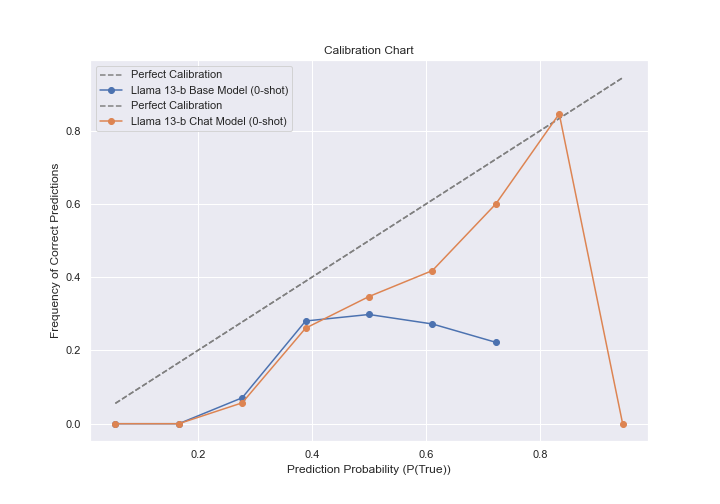
\includegraphics[width=1.3\textwidth]{figures/0-shot-13-b-chat-vs-13-b-hf}
         \caption{0-shot performance on MMLU dataset, we note calibration flattens fails to improve after 30\%, The model stall on accuracy unlike in multishot prompting scenario.}
         \label{fig:0-shot-MMLU}
     \end{subfigure}
     \hfill
     \begin{subfigure}[b]{0.49\textwidth}
         \centering
         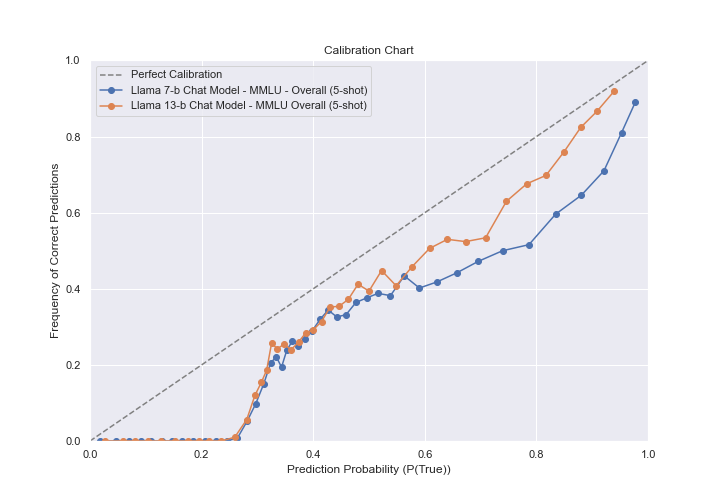
\includegraphics[width=1.3\textwidth]{figures/5-shot-MMLU.png}
         \caption{5-shot performance on MMLU on of chat models, we note that calibration improves with prompting for chat models, 13b-chat is better calibrated than 7b-chat}
         \label{fig:5-shot-logicqa}
     \end{subfigure}     
     
     \hfill
     \begin{subfigure}[b]{0.49\textwidth}
         \centering 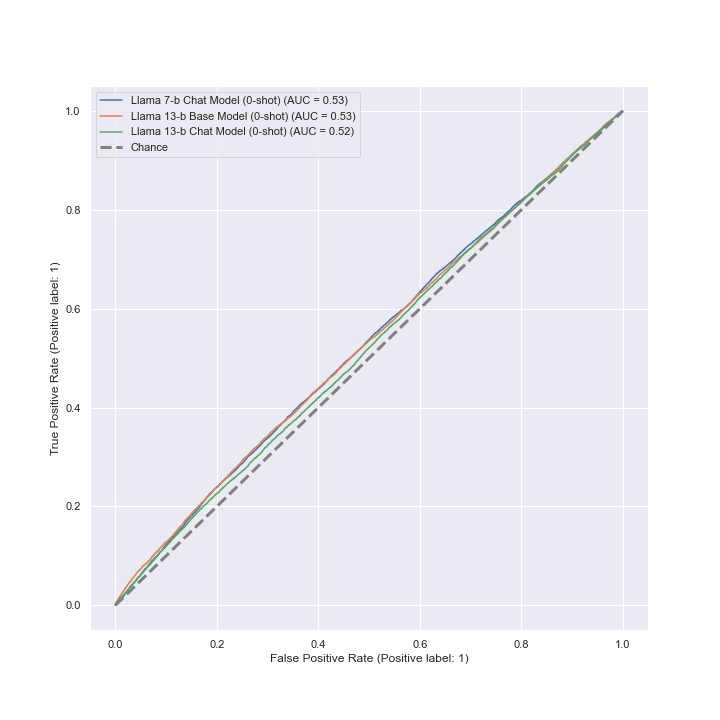
\includegraphics[width=0.9\textwidth]{figures/0-shot-MMLU-roc.png}
         \caption{0-shot MMLU shows poor classification performance},
         \label{fig:0-shot-MMLU}
    \end{subfigure} 
     \begin{subfigure}[b]{0.49\textwidth}
         \centering 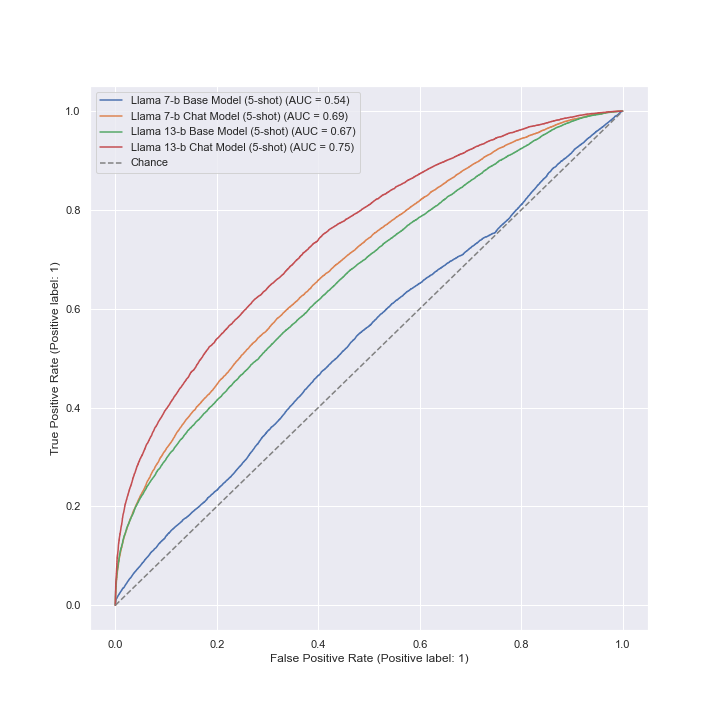
\includegraphics[width=0.9\textwidth]{figures/5-shot-MMLU-roc.png}
         \caption{5-shot ROC performance of Correct vs Rest classifier on 
         MMLU, we note that under prompting chat models accuracy and calibration shows marked improvement.},
         \label{fig:0-shot-MMLU}
    \end{subfigure} 
    
        \caption{Calibration Performance of Chat and Base models on the MMLU multiple choice question answering dataset.}
        \label{fig:three graphs}
\end{figure*}


\subsection{Model Calibration By Number of Parameters}

We compare the calibration of the Llama \cite{touvron2023llama} model 
7b-chat and 13b chat models for answering multiple choice questions in 
figure ... 

We note that that the calibration of the model while not perfect improves 
with the size of the model with the 13b-chat model being better calibrated 
and closer to the ideal calibration line than the 7b-chat model. Thus we 
note that models sizes improves not only the performance of the model but
the calibration of the model as well.


\begin{figure*}
     \centering
     \begin{subfigure}[b]{0.49\textwidth}
         \centering 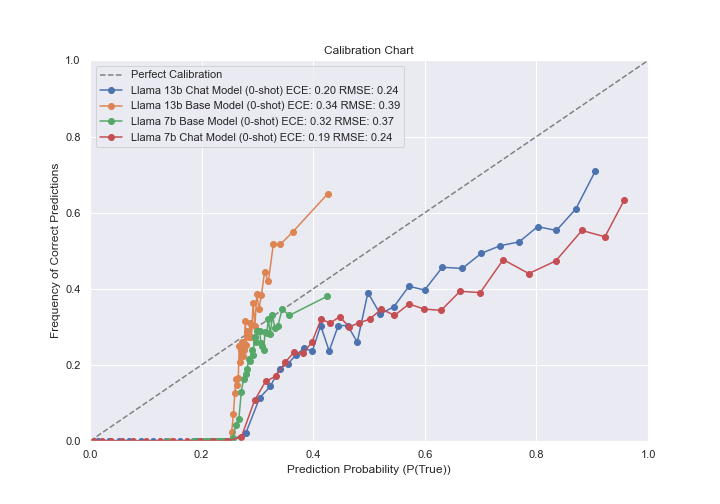
\includegraphics[width=1.3\textwidth]{figures/0-shot-logic-qa.png}
         \caption{0-shot performance on LogicQA, we note the base model under-predicts its performance.}
         \label{fig:0-shot-MMLU}
     \end{subfigure}
     \hfill
     \begin{subfigure}[b]{0.49\textwidth}
         \centering
         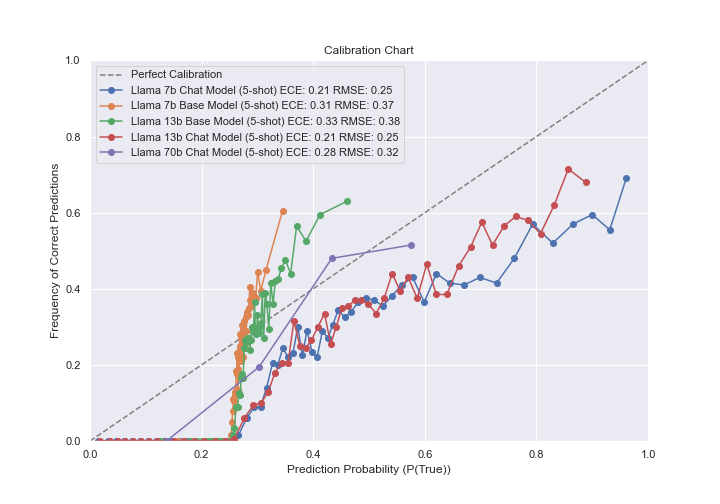
\includegraphics[width=1.3\textwidth]{figures/5-shot-logic-qa.png}
         \caption{5 shot performance on Logic QA. Chat models improve in calibration in 5-shot model, much like MMLU. Base models do not show any such improvement.}
         \label{fig:5-shot-logicqa}
     \end{subfigure}     
     
     \hfill
     \begin{subfigure}[b]{0.49\textwidth}
         \centering 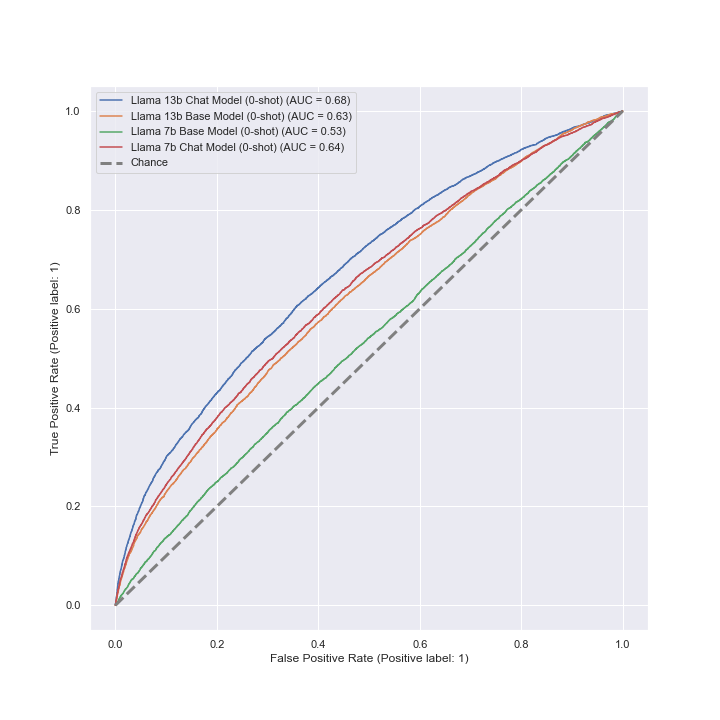
\includegraphics[width=0.9\textwidth]{figures/0-shot-logic-qa-roc.png}
         \caption{\textbf{0-shot Logic QA:} Bigger fine-tuned modes better \\accuracy},
         \label{fig:0-shot-MMLU}
    \end{subfigure} 
     \begin{subfigure}[b]{0.49\textwidth}
         \centering 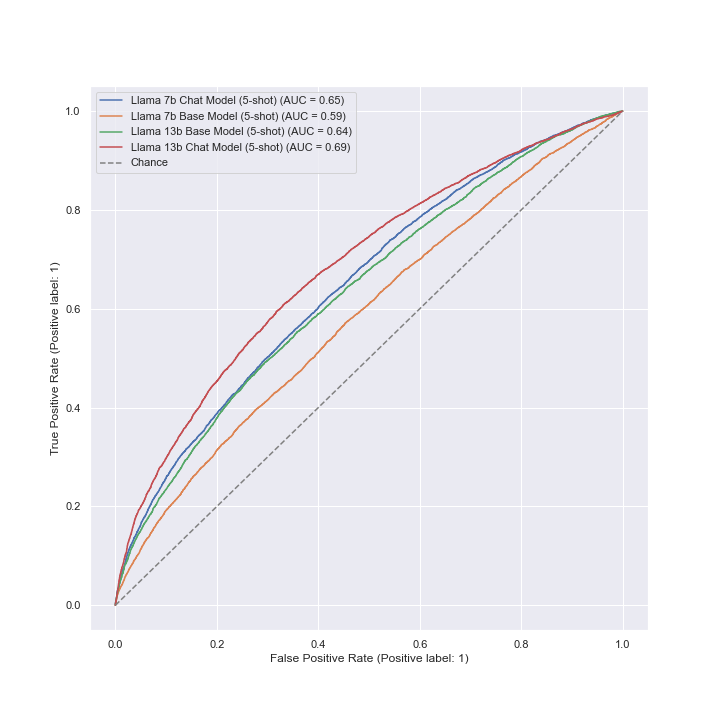
\includegraphics[width=0.9\textwidth]{figures/5-shot-logic-qa-roc.png}
         \caption{\textbf{5-shot Logic QA:}  note that we do not see significant differences in performance before and after prompting. Fine tuning however improves performance and calibration},
         \label{fig:0-shot-MMLU}
    \end{subfigure} 
     
     
        \caption{Calibration Performance of Chat and Base models on the LogicQA , logical question answering dataset}
        \label{fig:three graphs}
\end{figure*}

\begin{figure*}
     \centering
     \begin{subfigure}[b]{0.49\textwidth}
         \centering 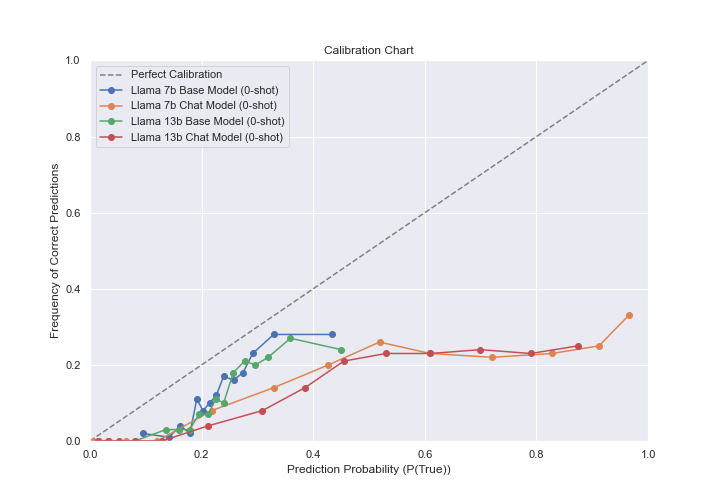
\includegraphics[width=1.3\textwidth]{figures/0-shot-truthful_qa.png}
         \caption{\textbf{0-Shot TruthfulQA:} We note that chat models suffer from overconfidence in 0-shot models, moreover model size fails to show significant improvement on TruthfulQA dataset}
         \label{fig:0-shot-truthfulqa}
     \end{subfigure}
     \hfill
     \begin{subfigure}[b]{0.49\textwidth}
         \centering
         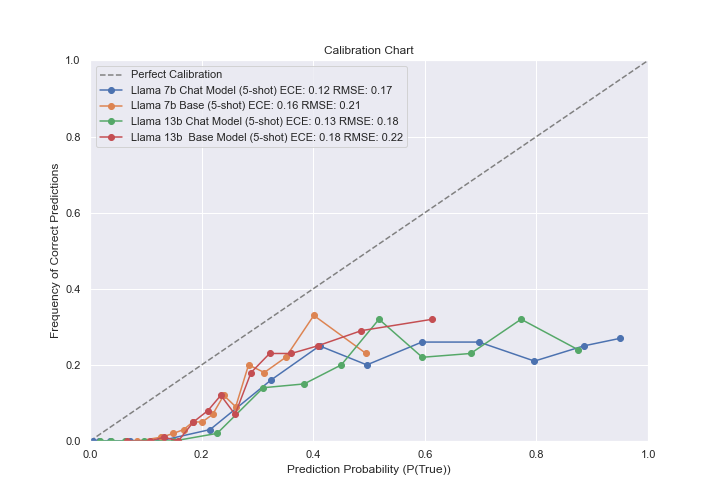
\includegraphics[width=1.3\textwidth]{figures/5-shot-TruthQA.png}
         \caption{\textbf{5-shot Truth QA:} Truthful QA finds chat models overconfident in thier prediction after fine-tuning. No large increase in accuracy or calibration is observed.}
         \label{fig:5-shot-truthfulqa}
     \end{subfigure}    
     
     \hfill
         \begin{subfigure}[b]{0.49\textwidth}
             \centering 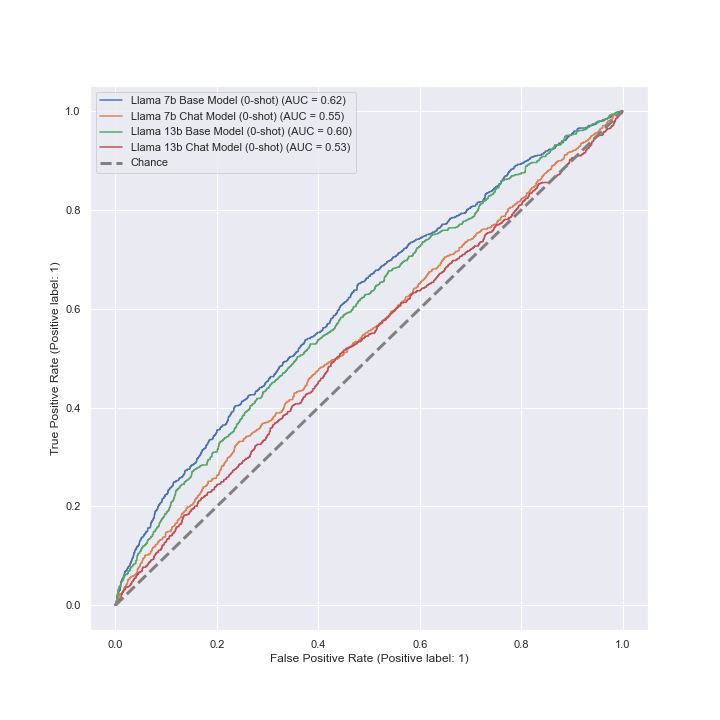
\includegraphics[width=0.9\textwidth]{figures/0-shot-truthful_qa-roc-roc.png}
             \caption{\textbf{0-shot TruthQA:} Base models marginally outperform fine-tuned chat models 
             in terms of accuracy},
             \label{fig:0-shot-MMLU}
        \end{subfigure} 
         \begin{subfigure}[b]{0.49\textwidth}
             \centering 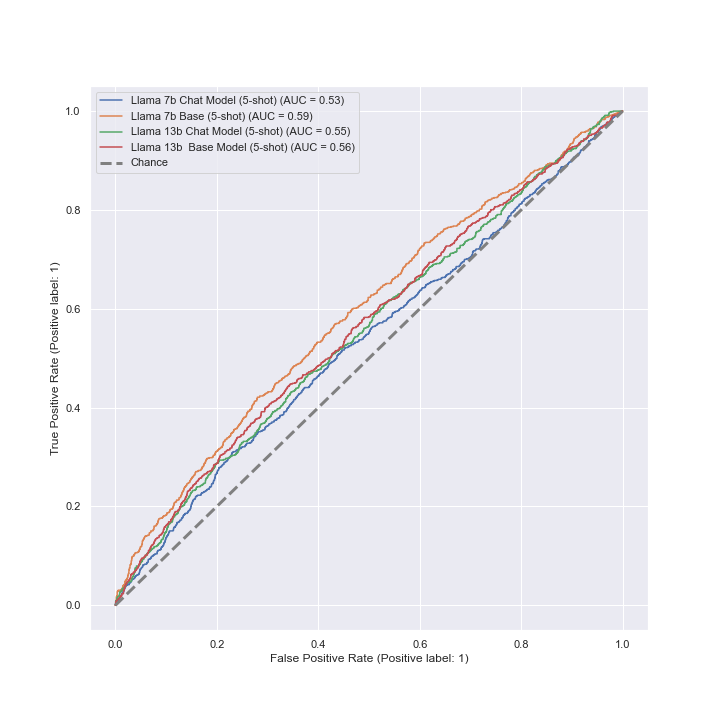
\includegraphics[width=0.9\textwidth]{figures/5-shot-TruthfulQA-roc.png}
             \caption{\textbf{5-shot Truthful QA:}  Multiple shot prompting worsens performance of fine-tuned models},
             \label{fig:0-shot-MMLU}
        \end{subfigure} 
         
         
     
        \caption{Calibration Performance of Chat and Base models on the Truthful QA , logical question answering dataset}
        \label{fig:three graphs}
\end{figure*}



\subsection{Model Calibration By Fine Tuning}  

We first note that fine tuning improves 0-shot calibration. For both 7b and 13b models as observed in 
Figure: \ref{fig:chat-vs-hf}. Where we note the chat model is closer to the ideal calibration line. Moreover we observe that 
multi-shot prompting as substantially improves the calibration of smaller 7-b model bringing it closer to calibration performance 13-b model used without prompting.


\subsection{Model Calibration By Subject Specialization}  

Another interesting phenomenon is seen for subject specialization on the MMLU bench mark. We note that calibration for 13b models  trends closer to ideal calibration line for more confident response with the exception of STEM fields where the calibration is substantially worse, having us conclude that the model 
is overconfident and incorrect on scientific questions.


\subsection{LogicQA}

LogicQA comprehensive dataset, named LogiQA, which is sourced from expert-written questions for testing human Logical reasoning. It consists of 8,678 QA instances, covering multiple types of deductive reasoning. Results show that state-of-the-art neural models perform by far worse than human ceiling. Our dataset can also serve as a benchmark for reinvestigating logical AI under the deep learning NLP setting. 


\subsection{TruthfulQA}

TruthfulQA is a benchmark to measure whether a language model is truthful in generating answers to questions. The benchmark comprises 817 questions that span 38 categories, including health, law, finance and politics. Questions are crafted so that some humans would answer falsely due to a false belief or misconception. To perform well, models must avoid generating false answers learned from imitating human texts.


\subsection{HumanEval}

\begin{figure}
  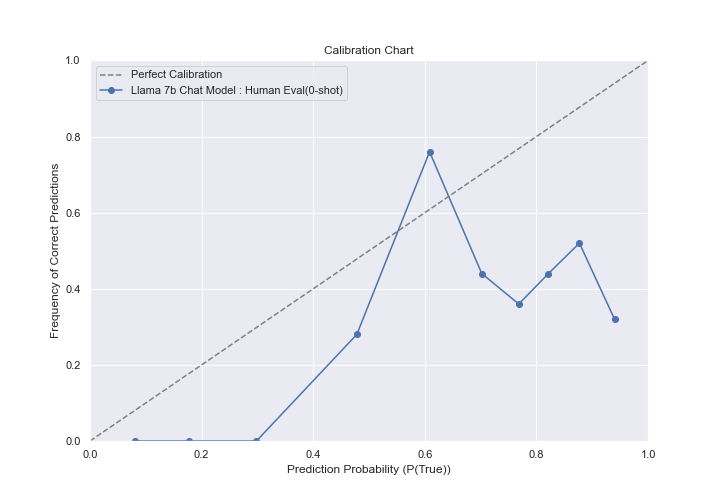
\includegraphics[width=0.5\textwidth]{figures/0-shot-7b-human-eval.png}
  \caption{We run a boolean model, to asses ability of model to judge if a proposed solution satisfies a requirement on human eval dataset.}
  \label{fig:human-eval-results}
\end{figure}

\subsection{GSM8k}

GSM8K (Grade School Math 8K) is a dataset of 8.5K high quality linguistically diverse grade school math word problems. The dataset was created to support the task of question answering on basic mathematical problems that require multi-step reasoning.

These problems take between 2 and 8 steps to solve. Solutions primarily involve performing a sequence of elementary calculations using basic arithmetic operations  to reach the final answer. A bright middle school student should be able to solve every problem: from the paper, "Problems require no concepts beyond the level of early Algebra, and the vast majority of problems can be solved without explicitly defining a variable." Solutions are provided in natural language, as opposed to pure math expressions. 

\subsection{Trivia}


\section{Results}

\section{Discussion}

\section{Conclusion}

In this study we attempted to study language model calibration 
under various conditions such as model size, fine tuning and  
task specialization. We found that we were able to replicate the 
observed  calibration behavior of closed models like GPT-3, and 
Claude on the open models like Llama 7b-chat and 13b-chat. 

We note that the calibration of the models  improved with the size 
of the model ...

While calibration is one aspect of querying model understanding it is 
certainly  not the only criteria for evaluating model understanding.  

Other criteria might include models' ability to reason step by step, 
and other demonstrate conceptual understanding by generalizing 
out of distribution. 

\section{Acknowledgements}

\section{References}

% Entries for the entire Anthology, followed by custom entries
\bibliography{anthology,custom}
\bibliographystyle{acl_natbib}

\appendix

\section{Appendix}
\label{sec:appendix}

This is a section in the appendix.

\end{document}
